\section{Dataset of Plastic Soup images}
\label{sec:Method-Data}
Because no dataset was available for this project, one was constructed by hand.


The dataset used in this project is made from short films by Bill MacDonnald\footnote{The videos are online on youtube: \url{www.youtube.com/007bmac}. Thank you Bill for letting me use your films in this research}.
Several of these clips consist of floating plastic from a viewpoint both above and below water.
These clips have been segmented in single frames and selected for use in this project.
A total of 37165 images were left to annotate.
The annotation has been done by my hand, classifying each image on viewpoint and if plastic or animals were visible.

To facilitate the annotation, a small Java-application was made.
With the use of several key-strokes, large amounts of image-data could be annotated with relative ease.
Even so, the annotation of the data took a considerable amount of time.

In total 20635 images show plastic only, 6972 images show animals only and 8502 images show both.
The above (16553) and below (20612) viewpoints were separated in two datasets, to train and test on both separately. 
In the above-set a total of 14588 images show plastic, 6341 images show animals and 863 images show none of both. In the below-set a total of 14549 images show plastic, 9133 images show animals and 193 images show none of both.
Figure \ref{fig:datasetimages} shows several examples of images in the dataset.
Both above and below water viewpoints are shown, as well as the labels the images were annotated with.

Because the images are constructed from films, many images are similar in appearance.
This fact should be taken in account when chances of overt-fitting occurs.
%Because many images are similar in appearance, fully training a CNN will be difficult.
%CNNs usually have millions of neurons, which makes the possibility of over-fitting on this dataset present.
%Moreover using a pre-trained neural network has other advantages, which are stated in section \ref{sec:Method-Algorithm}.
%==Tweede of derde keer dat je zegt dat ‘grote hoeveelheden data’ gebruikt zijn om CNNs te trainen. Maar hoeveel dan? En is dat echt nodig? Er worden ook CNNs geleerd op MNIST (60K afbeeldingen). Waarom kan dat niet? Of ga je dat laten zien mbv een experiment?

To evaluate the results of the pipeline, the dataset is divided in a train (70\%), validate (10\%) and test (20\%) set.
Because consecutive frames are similar, the division is done by using a pseudo-random randomise algorithm with each time the same seed.
Resulting in three sets of images that have a high distribution of the original data while remaining the same on each run.
The results of the algorithms can therefore be tested on accuracy with the amount of labels computed correctly.

\begin{figure}[h!tb]
\centering
\ifx\showfig\undefined
\def\iwith{.53\textwidth}
\centerline{
\begin{tabular}{rl}
\colorbox{red!70}{
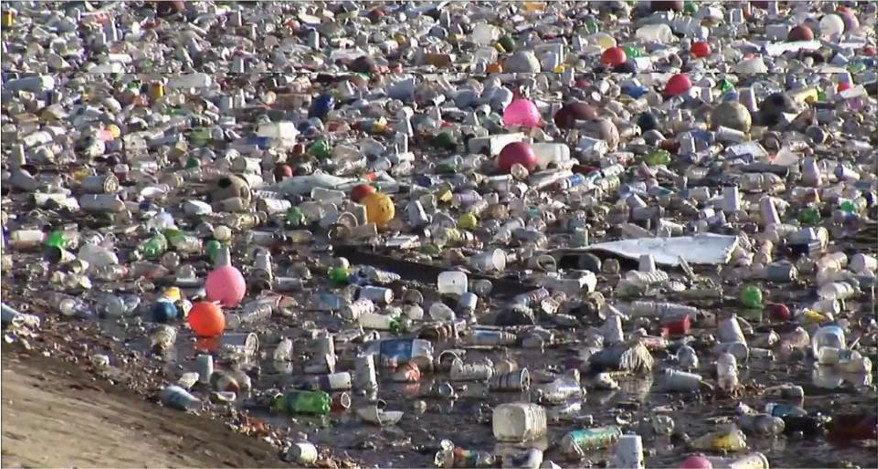
\includegraphics[keepaspectratio=true,width=\iwith]{images/matrix/253_01.jpg}}&
%
\colorbox{red!70}{
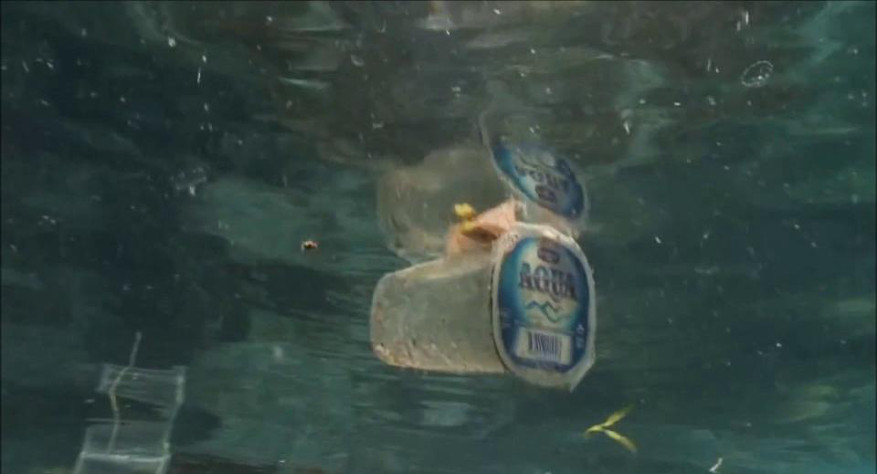
\includegraphics[keepaspectratio=true,width=\iwith]{images/matrix/20607_01.jpg}}\\
%
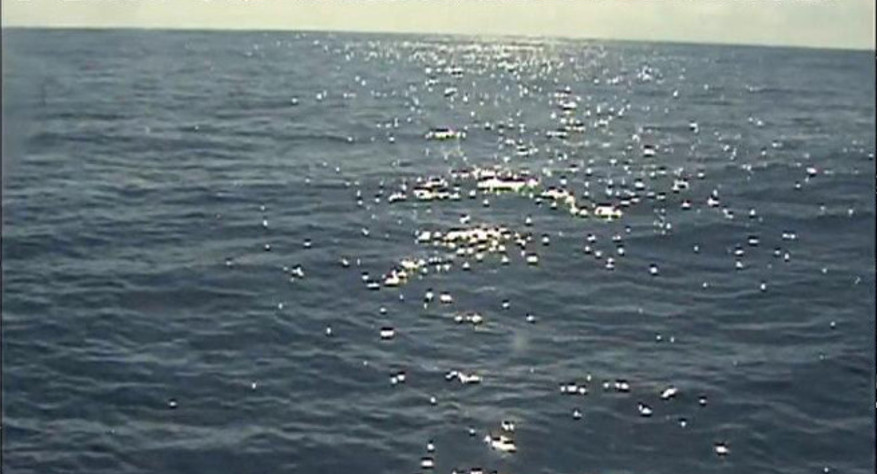
\includegraphics[keepaspectratio=true,width=\iwith]{images/matrix/299_00.jpg}&
%
\colorbox{green!80}{
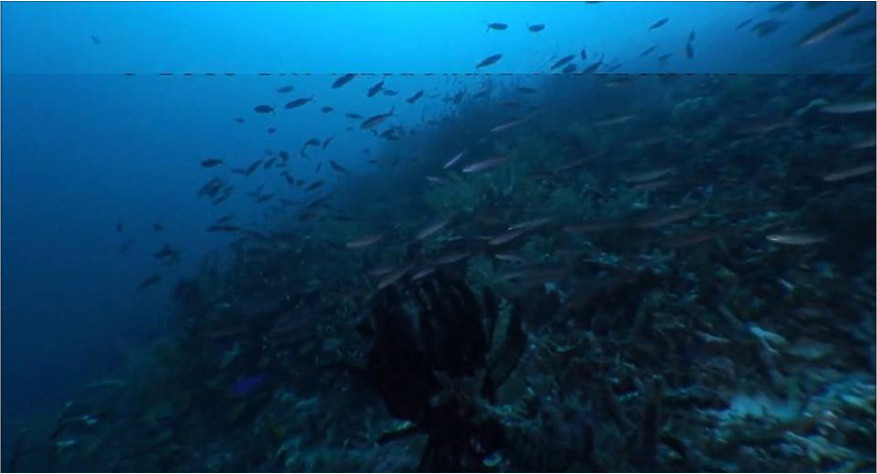
\includegraphics[keepaspectratio=true,width=\iwith]{images/matrix/2737_10.jpg}}\\
%
\colorbox{red!70}{\colorbox{green!80}{
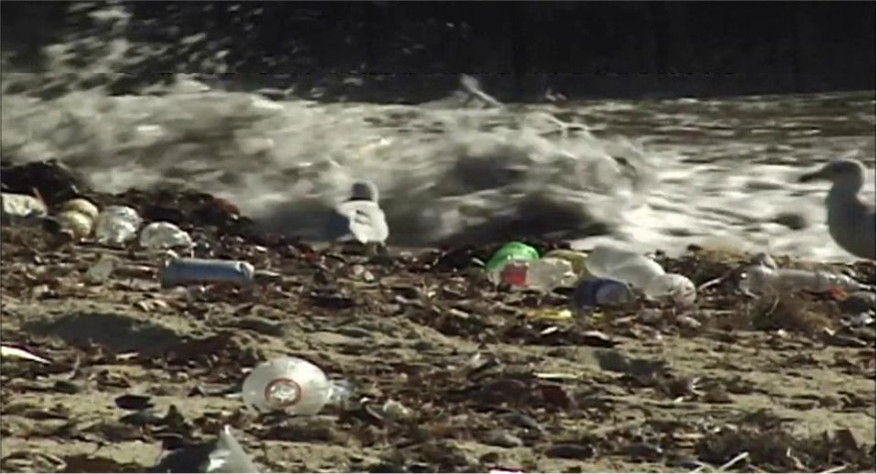
\includegraphics[keepaspectratio=true,width=\iwith]{images/matrix/31_11.jpg}}}&
%
\colorbox{red!70}{
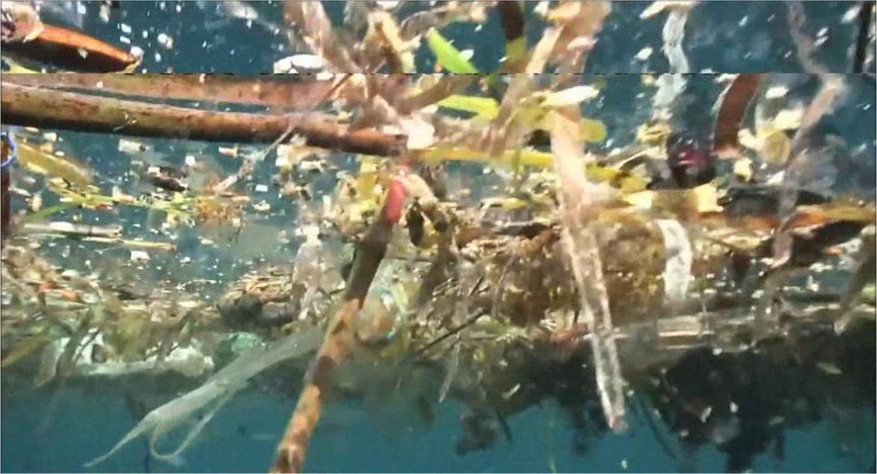
\includegraphics[keepaspectratio=true,width=\iwith]{images/matrix/4409_01.jpg}}\\
%
\colorbox{green!80}{
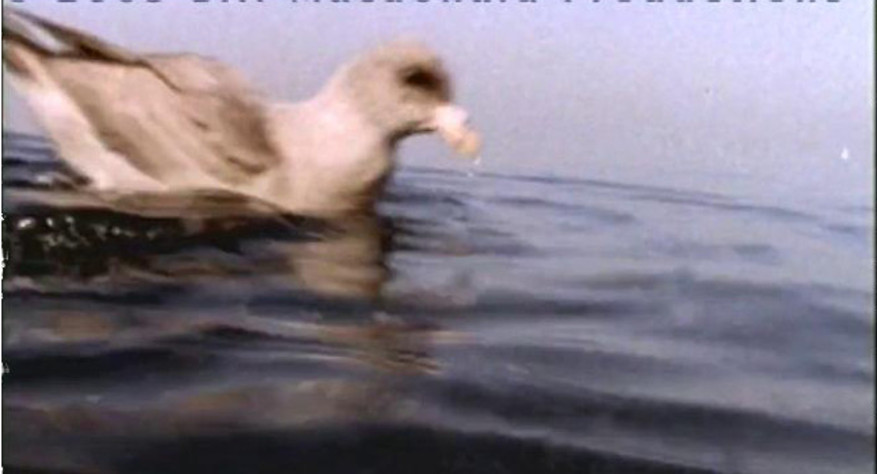
\includegraphics[keepaspectratio=true,width=\iwith]{images/matrix/401_10.jpg}}&
%
\colorbox{green!80}{
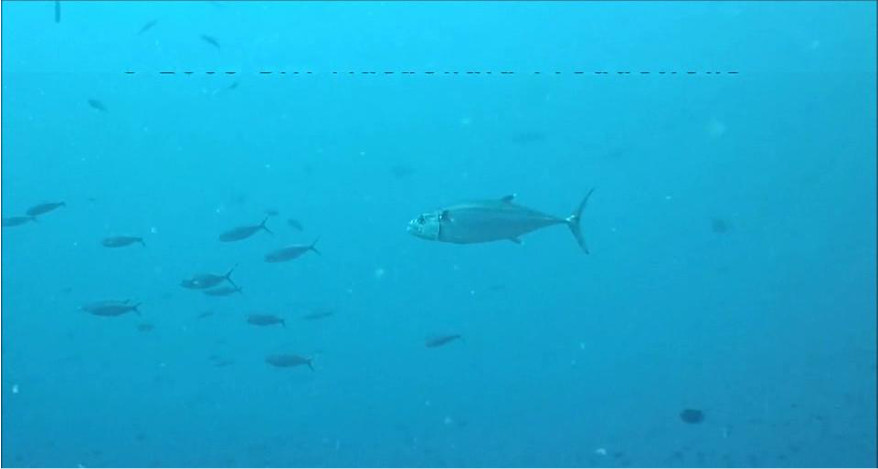
\includegraphics[keepaspectratio=true,width=\iwith]{images/matrix/5053_10.jpg}}\\
%
\colorbox{red!70}{\colorbox{green!80}{
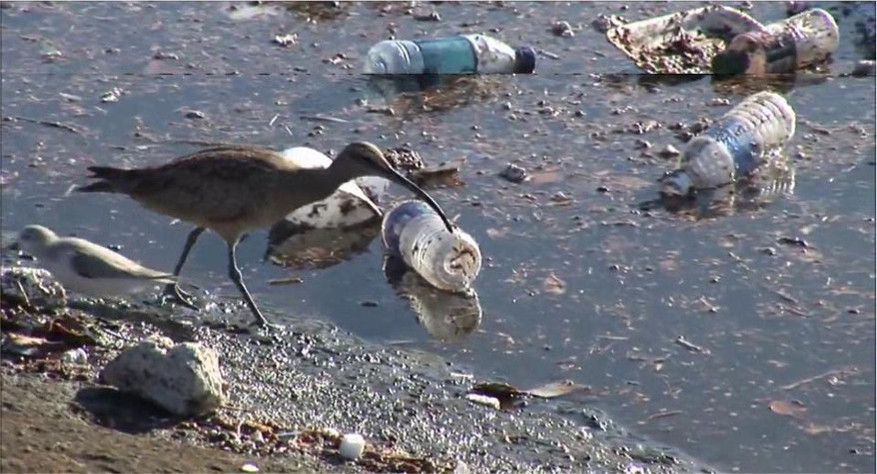
\includegraphics[keepaspectratio=true,width=\iwith]{images/matrix/701_11.jpg}}}&
%
\colorbox{red!70}{
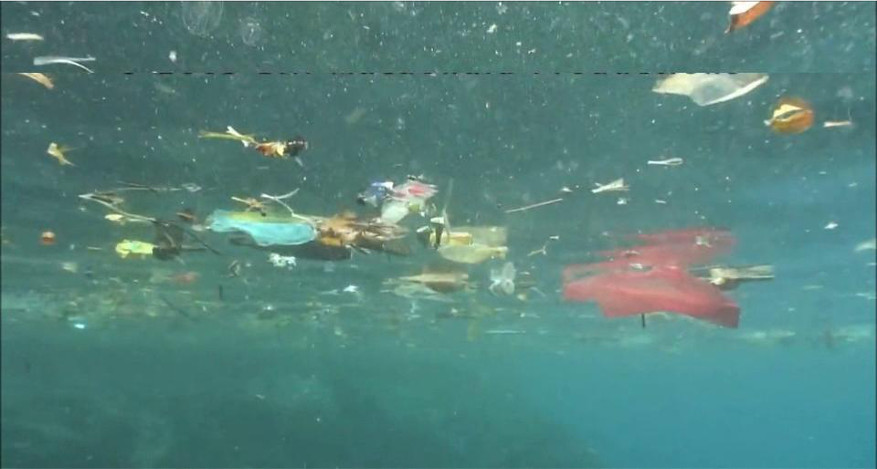
\includegraphics[keepaspectratio=true,width=\iwith]{images/matrix/6_01.jpg}}
\end{tabular}}
\fi
\caption{Several images from the dataset: Left images are from the above water viewpoint and right images are from below water. A red border indicates an image classified as showing plastic, where a green border indicates an image classified as showing animals.}
\label{fig:datasetimages}
\end{figure}